\subsubsection{UC 5 - \textit{Logout}}
\begin{figure}[H]
    \vspace{2em}
    \centering
    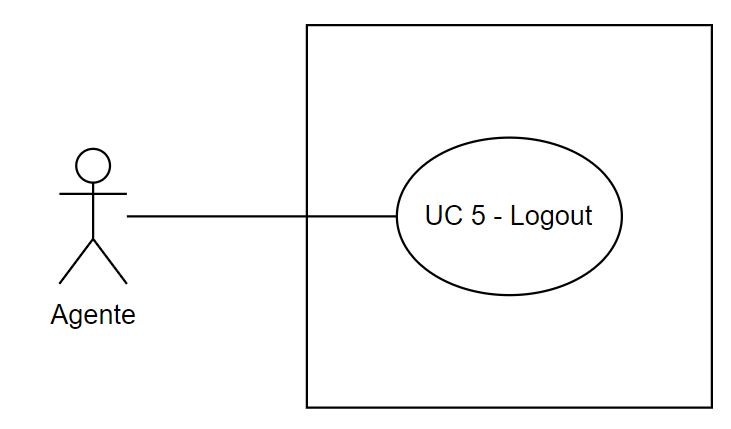
\includegraphics[width=0.75\columnwidth]{img/usecase/UC 5.png}
    \caption{\textit{Use Case} 5: \textit{Logout}}
    \label{fig:uc_5}
\end{figure}

\begin{usecase}{ 5}{\textit{Logout}}
    \usecaseactors{Agente.}
    \usecasedesc{L'agente effettua la procedura di \textit{logout}.}
    \usecasepre{L'agente, dalla \texttt{Homepage Agenti}, cliccando nell'apposito menu il pulsante "\textit{Account}", si 
                sposta nella pagina \texttt{Account}.}
    \usecasepost{L'agente ha effettuato il \textit{logout} e torna un utente non autenticato. 
                 L'agente viene spostato alla pagina di \textit{login}.}
    \usecasescen{
        \begin{itemize}
            \item L'agente si trova nella \texttt{Homepage Agenti};
            \item L'agente preme il pulsante "\textit{Account}" dal menu;
            \item L'agente viene spostato nella pagina \texttt{Account};
            \item L'agente effettua il \textit{logout};
            \item L'agente torna un utente non autenticato;
            \item L'agente viene spostato alla pagina di \textit{login}
        \end{itemize}}
    \label{uc:uc_5}
\end{usecase}